% !TEX root = DauceAlbigesPerrinet2020.tex
% !TEX encoding = UTF-8 Unicode
% -*- coding: UTF-8; -*-
% vim: set fenc=utf-8
% !TEX spellcheck = en-US


\section{Setup}
\label{sec:principles}
%=================================================================
%=================================================================
%------------------------------%

\begin{figure}[t!]%[b!]%%[p!]
	\centering{	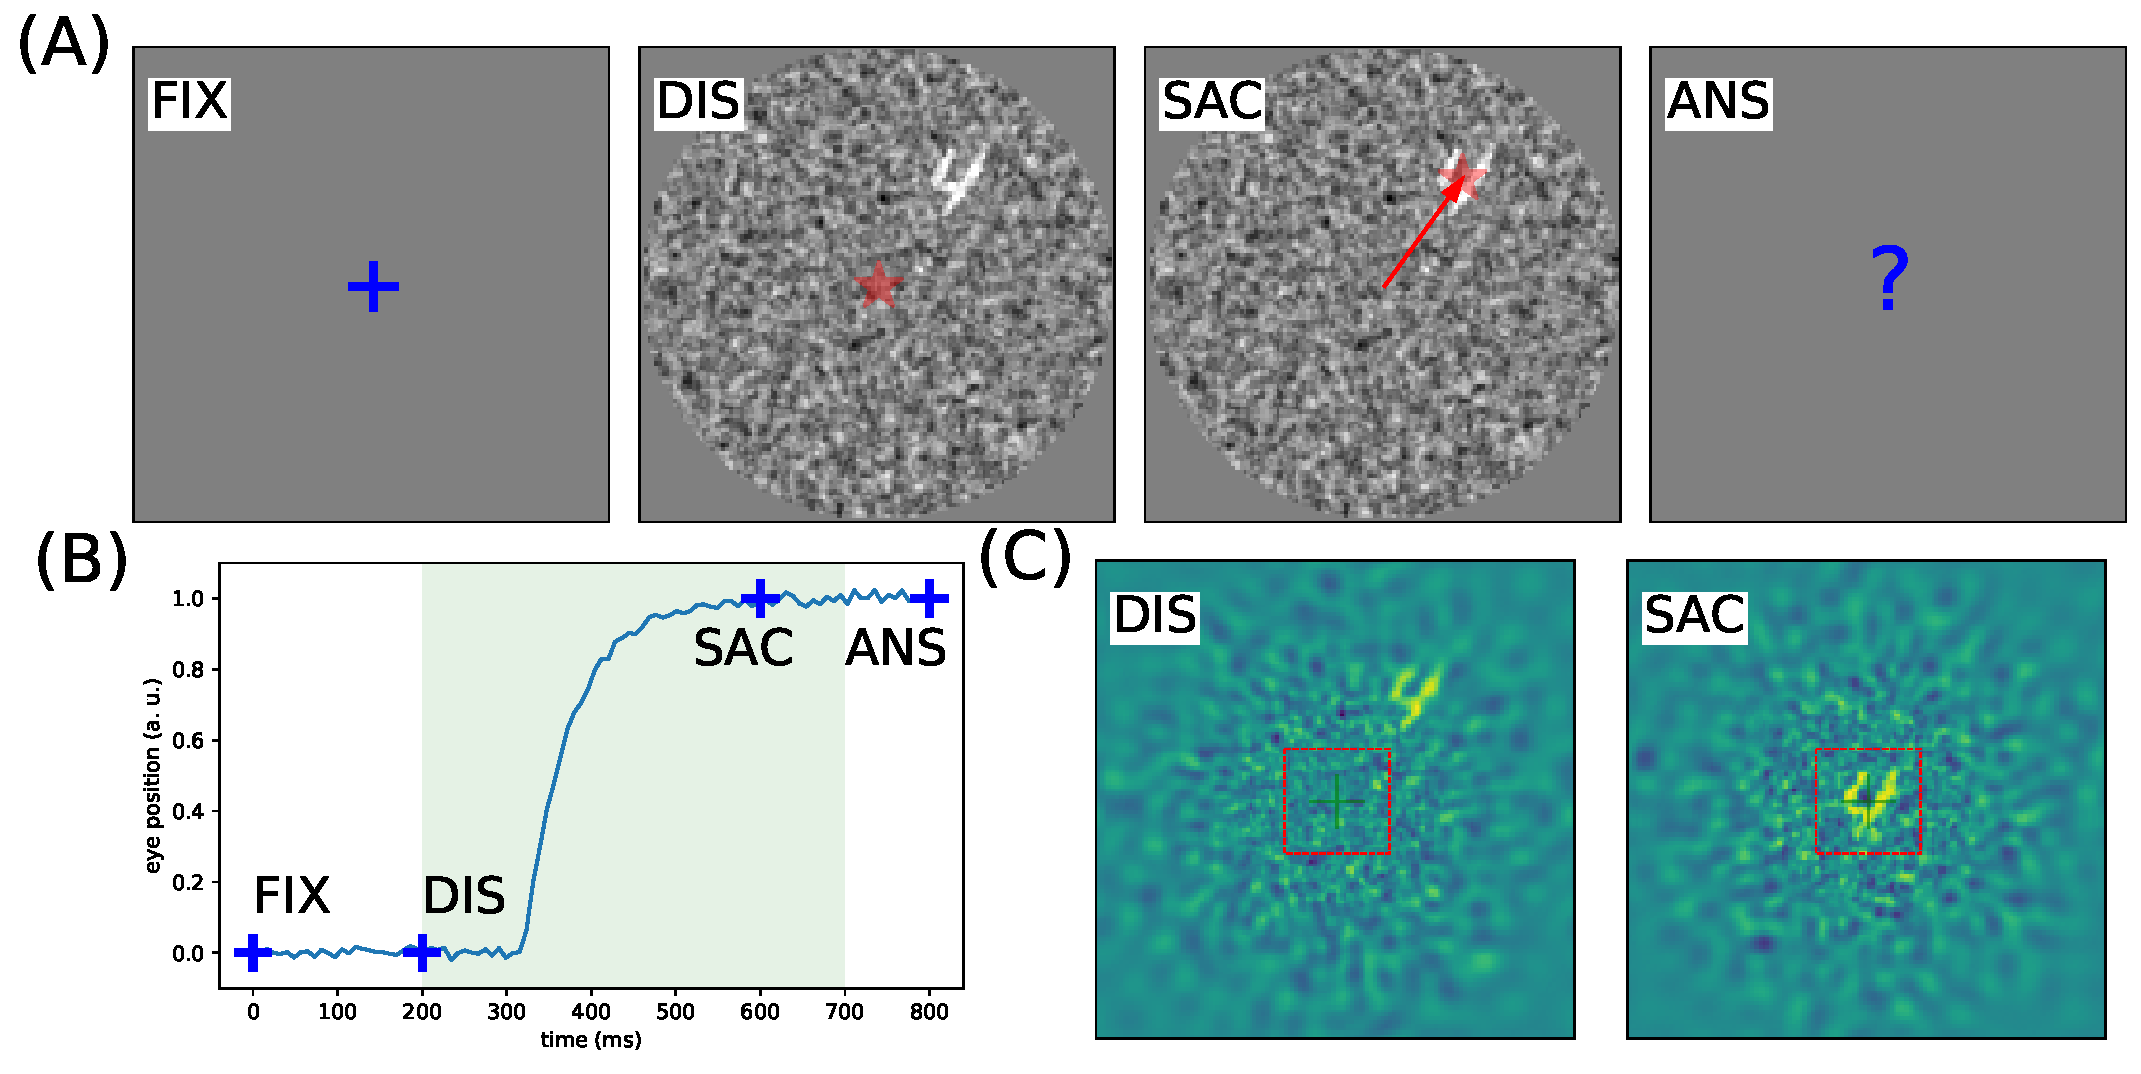
\includegraphics[width=\linewidth]{fig_intro}} %
	\caption{%
		{\bf Problem setting}: In generic, ecological settings, when searching for one target (from a class of targets) in a cluttered environment the visual system is bound with an action selection problem. It is synthesized in the following virtual experiment: %
		\A After a fixation period \FIX\ of $200~\ms$, an observer is presented with a luminous display \DIS\ showing a single target from a known class (here digits) put at a random position within the field of view. The display is presented for a short period of $500~\ms$ (light shaded area in B), that is enough to perform at most one saccade on the potential target (\SAC , here successful). Finally, the observer has to identify the digit by a keypress \ANS. \emph{NB}: the target contrast is here enhanced to $100\%$ for a better readability. %
		\B Prototypical trace of a saccadic eye movement to the target position. In particular, we show the fixation window \FIX\ and the temporal window during which a saccade is possible (green shaded area). %
		\C Simulated reconstruction of the visual information from the internal retinotopic map at the onset of the display \DIS\ and after a saccade \SAC , the dashed red box indicating the foveal region. The task does not consist in inferring the location of the target, but rather to infer an action that may provide relevant pixels at the center of fixation, allowing to identify the target's category. By comparison with the external display (see A), the action is processed from log-polar coefficients, representing a focal sample of the total visual field.
		Controlling the clutter and reducing the contrast of the digit allows to monitor the task difficulty.
		 }%
	\label{fig:intro} %
\end{figure}%
%%------------------------------%

\subsection{Experimental design}

In order to implement our visual processing setup,
we provide a simplified visual environment toward which a visual agent can act on.
This visual search task is formalized and simplified in a way reminiscent to classical psychophysic experiments: an observer is asked to classify digits (for instance as taken from the MNIST dataset, as introduced by~\cite{Lecun1998}) as they are shown with a given size on a computer display.
However, these digits can be placed at random positions on the display, and visual clutter is added as a background to the image (see Figure~\ref{fig:intro}-A).
In order to vary the difficulty of the task, different parameters are controlled, such as the target eccentricity, the background noise period and and the signal/noise ratio (SNR).
The agent initially fixates the center of the screen. Due to the peripheral clutter, he needs to explore the visual scene through saccades to provide the answer. He controls a foveal visual sensor that can move over the visual scene through saccades (see Figure~\ref{fig:intro}-B). When a saccade is actuated, the center of fixation moves toward a new location, which updates the visual input (see Figure~\ref{fig:intro}-C).
The lower the SNR and the larger the initial target eccentricity, the more difficult the identification. There is a range of eccentricities for which it is impossible to identify the target from a single glance, so that a saccade is necessary to issue a proper response.
%We will define a neural network which implements this control process.
%The agent aims at understanding the visual scene, here identifying both the target position and identity from visual samples.
This implies in general that the position of the object may be detected in the first place in the peripheral clutter before being properly identified.

This setup provides the conditions for a separate processing of the visual information.
%, with visuo-spatial information extracted from the peripheral clutter, and object detailed shape and identity extracted through central foveal examination.
%Indeed, in order to analyze a complex visual scene, two kinds of processing are interleaved.
On the one side, the detailed information present at the center of fixation needs to be analyzed to provide specific environmental cues.
%, that is the region of interest currently processed.
On the other side, the full visual field, i.e. mainly the low resolution part surrounding the fovea, needs to be processed in order to identify regions of interest that deserve fixation. This basically means making a choice of “what’s interesting next”. The actual content of putative peripheral locations does not need to be known in advance, but it needs to look interesting enough, and of course to be reachable by a saccade. This is reminiscent of the What/Where visual processing separation observed in monkeys and humans ventral and dorsal visual pathways~\cite{mishkin1983object}.

\begin{figure}[t!]%%[p!]
	\centering{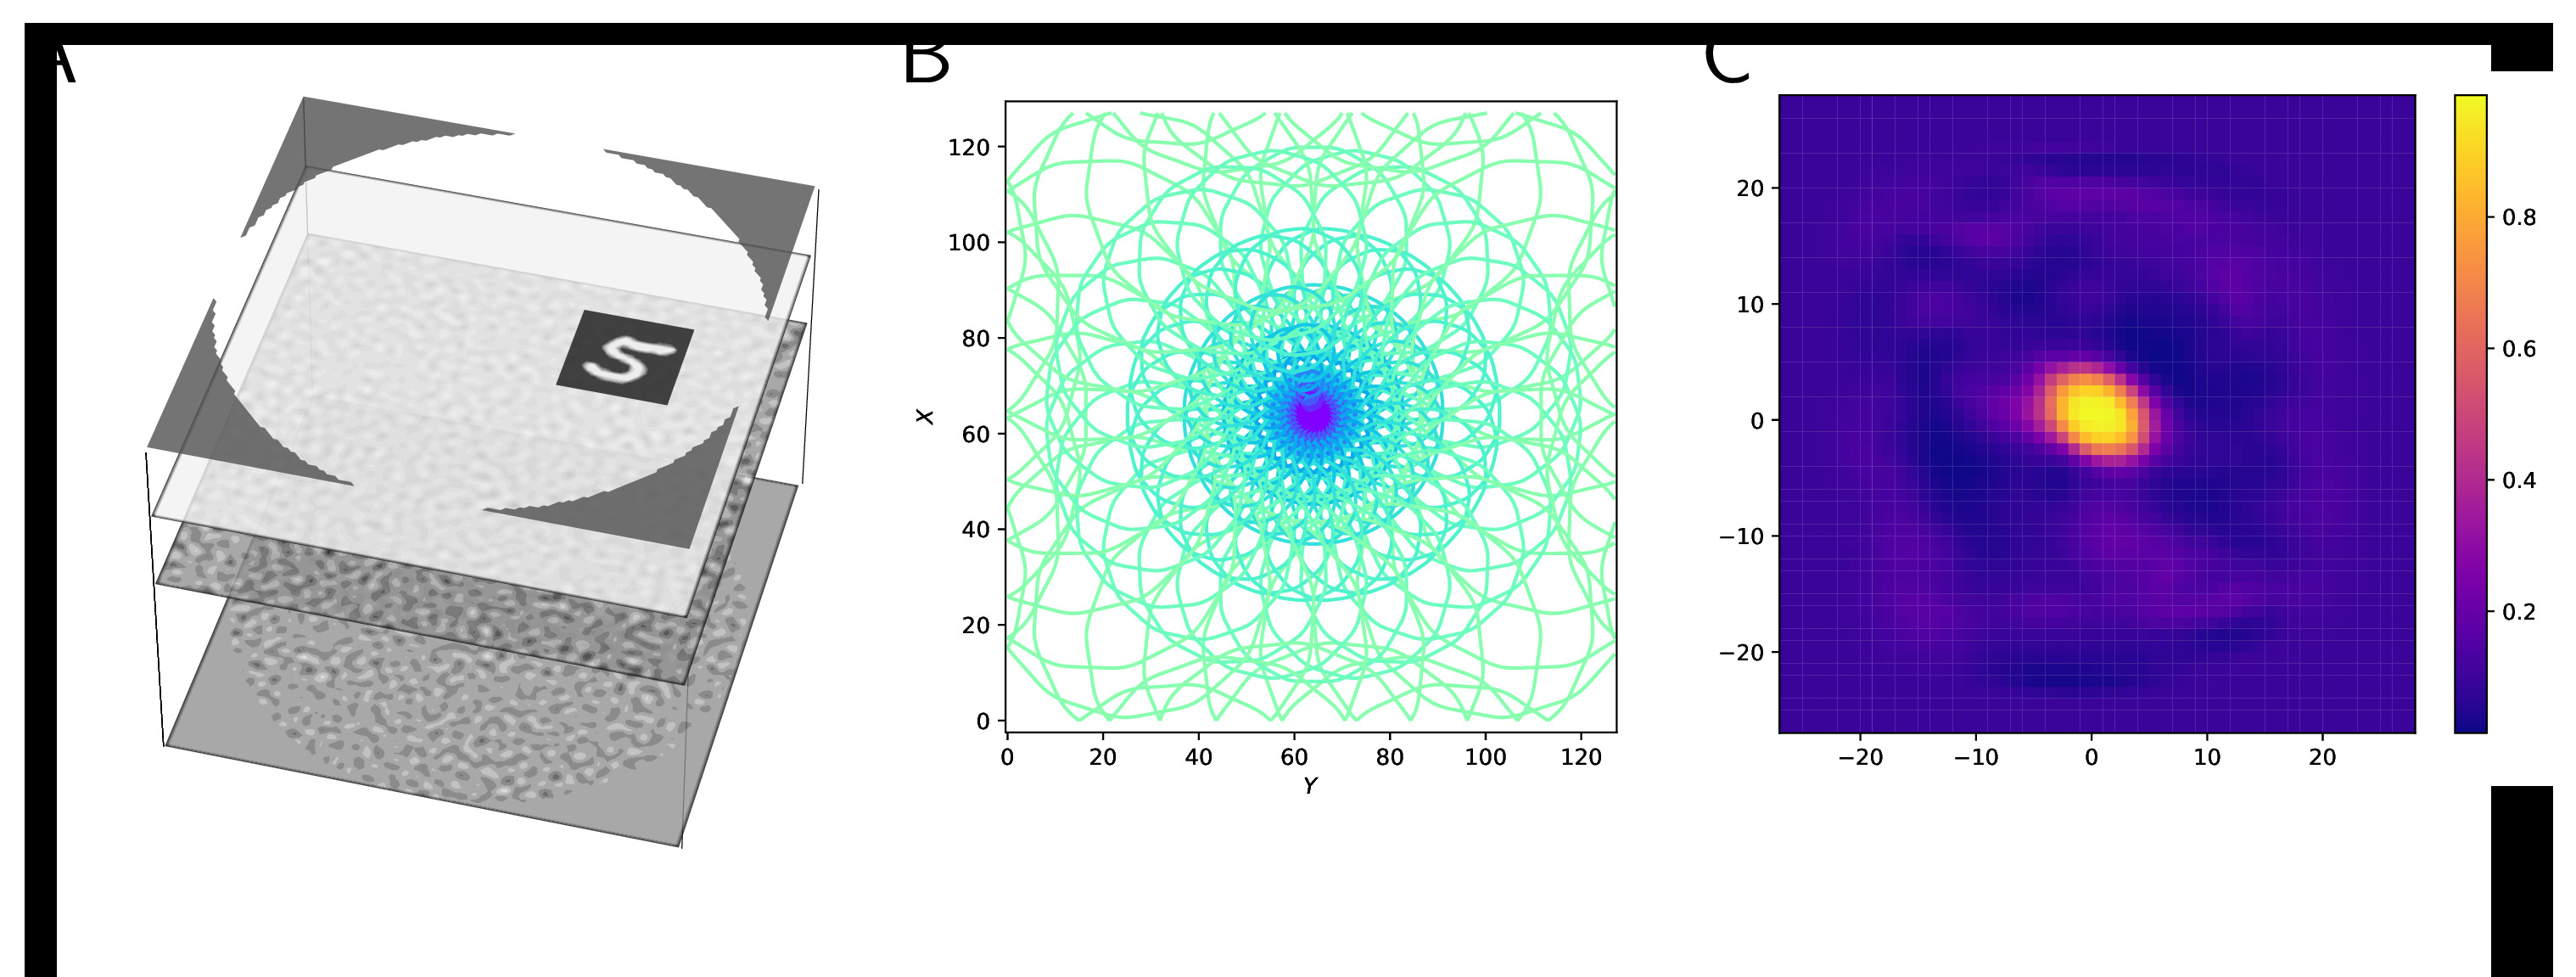
\includegraphics[width=\linewidth]{fig_methods}}
	\caption{%
		{\bf Computational graph}. From the anatomy of the primary visual pathways, we define two streams of information, one stream for processing the central pixels only (``What''?), the other for localizing a target in the image ( ``Where''?) by processing the periphery with a log-polar encoding. The two streams converge toward a decision layer that compares the central and the peripheral accuracy, in order to decide whether to issue a saccadic or a categorical response. If a saccade is realized, then the center of vision is displaced toward the region that shows the highest accuracy on the accuracy map.
		\A The visual display is constructed the following way: first a $128\times 128$ natural-like background noise is generated, characterized by noise contrast, mean spatial frequency and bandwidth~\cite{Sanz12}. Then a circular mask is put on. Last, a sample digit is selected from the MNIST dataset (of size $28\times 28$), rectified, multiplied by a contrast factor and overlaid on the background at a random position (see another example in Figure~\ref{fig:intro}-A, \DIS ). %
		\B The visual display is then transformed in 2 sensory inputs: (i)~a $28\times 28$ central foveal-like snippet is fed to a classification network (``What'' pathway) and (ii)~a log-polar set of oriented visual features is fed to the ``Where'' pathway. This log-polar input is generated by a bank of filters whose centers are positioned on a log-polar grid and whose radius increases proportionally with the eccentricity. %
		\C The ``What'' network is implemented using the three-layered LeNet neural network~\cite{Lecun1998}, while the ``Where'' network is implemented by a three-layered neural network consisting of the retinal log-polar input, two hidden layers (fully-connected linear layers combined with a ReLU non-linearity) with $1000$ units each and a collicular-like accuracy map at the output. This map has a similar retinotopic organization and predicts for the accuracy of the hypothetical position of a saccade. To learn to associate the output of the network with the ground truth, supervised training is performed using back-propagation with a binary cross entropy loss.
		\D
		% {\color{red} \textbf{rev 2} In Figure 2 part (D), a stopping condition is explicitly given. However, this rule is not explicitly mentioned in the text. The relevant part is the “Concurrent action selection” on page 16. This section should be improved for clarity. And, explicit connections should be drawn to Figure 2.}
		%Once both networks are trained,
		For a given display to the dual network generates two sensory inputs and two accuracy outputs. If the predicted accuracy in the output of the ``Where'' network is higher than that predicted in the ``What'' network, the position of maximal activity in the ``Where'' pathway serves to generate a saccade which shifts the center of gaze. Else, we interrupt the visual search and classify the foveal image using the ``What'' pathway such as to give the answer~(\ANS ). %
		\label{fig:methods}}%
\end{figure}%
%%------------------------------%


\subsection{Accuracy map training}

Modern parametric classifiers are composed of many layers (hence the term ``Deep Learning'') that can be trained through gradient descent over arbitrary input and output feature spaces. The ease of use of those tightly optimized training algorithms is sufficient to allow for the quantification of the difficulty of a task through the failure or success of the training.
For our specific problem, the simplified anatomy of the agent is composed of two separate pathways for which each processing is realized by such a neural network (see Figure~\ref{fig:methods}). The proposed computational architecture is connected in a closed-loop fashion with a visual environment, with the capacity to produce saccades whose effect is to shift the visual field from one place to another. Crucially, the processing of the visual field is done through distinct pathways, each pathway being assumed to rely on different sensor morphologies. By analogy with biological vision, the target identification is assumed to rely on the very central part of the retina (the fovea), that comes with higher density of cones, and thus higher spatial precision. In contrast, the saccade planning should rely on the full visual field, with peripheral regions having a lower sensor density and a lesser sensitivity to high spatial frequencies. A first classifier is thus assigned to process only the pixels found at the center of fixation, while a second one processes the full visual field with a retina-mimetic central log-polar magnification. The first one is called the ``What'' network, and the second one is the ``Where'' network (see Figure~\ref{fig:where} for details). They are both implemented in \texttt{pytorch}~\cite{NEURIPS2019_9015}, and trained with gradient descent over multiple layers.

In a stationary condition, where the target's position and identity do not change over time, each saccade thus provides a new viewpoint over the scene, allowing to form a new estimation of the target identity.
%Examining the current visual field $x$ allows to form two hypotheses, namely $p(U|x)$ and $p(Y|x)$. It may happen, however, that the current inferences may not be accurate enough and there may be a ``better'' eye direction from which more evidence could be grabbed, i.e. it may be worth issuing a saccade so that $p(U'|x')$ and $p(Y|x')$ should be more accurate.
Following the active inference setup~\cite{Najemnik05, Friston12}, we assume that, instead of trying to detect the actual position of the target, the agent tries to maximize the scene understanding benefit of doing a saccade. The focus is thus put on action selection metric rather than spatial representation.
This means in short estimating how accurate a categorical target classifier will be after moving the eye.
%action selection can be interpreted as choosing the saccade that should provide the best target identity estimate.
In a full setup, predictive action selection means first predicting the future visual field $x'$ obtained at the center of fixation, and then predicting how good the %$p(U|x)$ and $p(Y|x)$
estimate of the target identity $y$, i.e. $p(y|x')$, will be at this location.
% a full sequence of operations comprises first an initial visual examination through the where and the what pathways. This . followed by ($ii$) a decision, ($iii$) a saccade realization and ($iv$) a second visual examination that should finally ($v$) determine the category of the target.
%It is worth noting that active inference needs either the current identity $y$ or the current eye direction $u$ to be readable from the present view, in order to effectively predict future inferences, through computationally intensive predictions.
In practice, %modeling the full sequence of operations that lead to estimate %both $p(U'|x')$ and $p(Y|x')$
%the future $u$ and $y$
%means predicting
predicting a future visual field over all possible saccades is too computationally expensive. %in the case of large visual fields.
Better off instead is to record, for every context $x$, the improvement obtained in recognizing the target after a sequence of saccades $a, a', a'', \ldots$.
If $a$ is a possible saccade and $x'$ the corresponding future visual field, the result of the central categorical classifier over $x'$ can either be correct ($1$) or incorrect ($0$).
If this experiment is repeated many times over many visual scenes, the probability of correctly classifying the future visual field $x'$ from $a$ is a number between $0$ and $1$, that reflects the proportion of correct and incorrect classifications.
% This means forming an \emph{accuracy map} from the current view. This is the essence of the \emph{sampling-based metric prediction} that we develop here.
The putative effect of every saccade can thus be condensed in a single number, the \emph{accuracy}, that quantifies the final benefit of issuing saccade $a$ %regarding the target identity, both assuming $p(U|\boldsymbol{x})$ and $p(Y|\boldsymbol{x})$
from the current observation $x$. %
% when issuing a saccade $a$ after seeing $\boldsymbol{x}$ (the initial visual field).
%It more or less corresponds to inferring the true target identity $\hat{y}$, i.e. $p(\hat{y}|x')$, including the update of the eye direction, that is a sample of the ``real'' generative process.
%In a biological setting, this would be acchieved for instance by catch-up saccades that would scan the area neighboring the saccade that was actually issued.
 Extended to the full action space $A$, this forms an accuracy map that should monitor the selection of saccades. %after processing the visual input,
This accuracy map can be trained by trials and errors, with the final classification success or failure used as a teaching signal. Our main assumption here is that such a \emph{predictive accuracy map} is at the core of a realistic saccade-based vision systems, with the ``What'' network playing the role of a ``critic'' over the output of the ``Where'' network (see~\cite{sutton1998reinforcement}).
%Consistently with a baseline approach that would predict for all possible gaze directions over an image, this map should moreover be organized radially to preserve the initial retinotopic organization.
%, as exemplified by a retinotopic map. The map , preserving the initial retinotopic organization. %with high predicted accuracies reflecting a high probability of target presence at given locations.

Each task is assumed to be realized in parallel through the ``What'' and the ``Where'' pathways by analogy with the ventral and dorsal pathways in the brain (see figure~\ref{fig:methods}).
From the active inference standpoint, the separation of the scene analysis in those two independent tasks relies on a simple ``Naïve Bayes'' assumption (see Methods). %A first task consists in identifying the target (namely inferring $y$ from $x$) and a second task consists in localizing the target (namely inferring $u$ from $x$).
%\bf [ref needed]. \emph{Note that %from the retinotopic projection of the visual information,
%this independence is conditional on action: both pathways should update their beliefs upon decisions made in each respective pathway {\bf (je ne comprends pas bien cette phrase?)}}}\fi.
%However, we will here simplify the setting by considering only one possible saccade.
The operations that transform the initial primary visual data should preserve the initial retinotopic organization, so as to form a final retinotopic accuracy map. % (see figure~\ref{fig:methods}C).
Accordingly with the visual data, the retinotopic accuracy map may thus provide more detailed accuracy predictions in the center, and coarser accuracy predictions in the periphery.
%and telling how accurate the categorical classifier will be after the saccade is carried out~\cite{Dauce18}. %The set of all possible saccade predictions should
Finally, each different initial visual field may bring out a different accuracy map, indirectly conveying information about the target retinotopic position.
A final action selection (motor map) should then overlay the accuracy map through a winner-takes-all mechanism (see figure~\ref{fig:methods}-D), implementing the saccade selection in biologically plausible way, as it is thought to be done in the superior colliculus, a brain region responsible for oculomotor control~\cite{sparks1987sensory}.
The saccadic motor output showing a similar log-polar compression than the visual input, the saccades should be more precise at short than at long distance (and several saccades may be necessary to precisely reach distant targets). %
%
Each network is trained and tested separately. Because the training of the ``Where'' pathway depends on the accuracy given by the ``What'' pathway (and not the reverse), we trained the latter first, though a joint learning also yielded similar results. % TODO : à vérifier
Finally, these are evaluated in a coupled, dynamic vision setup.



%=================================================================
\section{Results}
\label{sec:results}
%=================================================================



%------------------------------%
\begin{figure}[t!]%%[p!]
	%\flushleft{\bf (A) \hspace{4.2cm} (B) \hspace{2cm} (C) \hspace{4cm} (D)\hspace{6cm}}
	\centering{{\bf a.} \hspace{1.6cm} {\bf b.} \hspace{1.6cm} {\bf c.} \hspace{1.6cm} {\bf d.} \hspace{1.6cm} {\bf e.}}
	\centering{\A\includegraphics[width=.9\linewidth]{CNS-saccade-8.png}}
	\centering{\B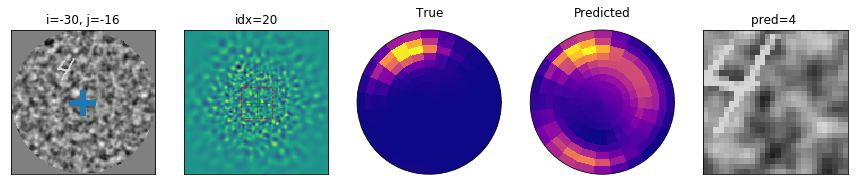
\includegraphics[width=.9\linewidth]{CNS-saccade-20.png}}
	\centering{\C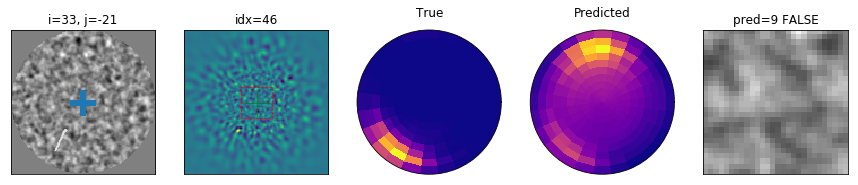
\includegraphics[width=.9\linewidth]{CNS-saccade-46.png}}
	\centering{\D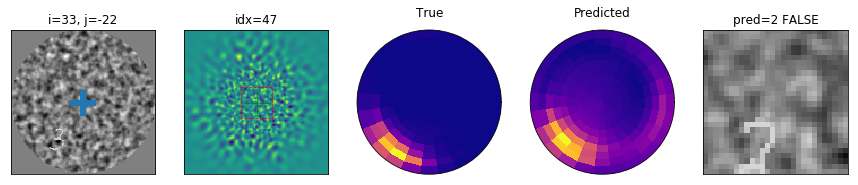
\includegraphics[width=.9\linewidth]{CNS-saccade-47.png}}
	\centering{\E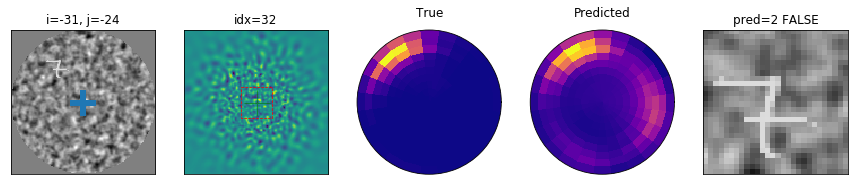
\includegraphics[width=.9\linewidth]{CNS-saccade-32.png}}
	% \includegraphics[]{../../2019-07-15_CNS/figures/CNS-saccade-8.png} % TRUE
	\caption{
		{\A-- \E Representative active vision samples after training}: \A-- \B classification success samples, \C-- \E classification failure samples. Digit contrast set to $70\%$. From left to right: {\bf a.}~The initial 128$\times$128 visual display, with blue cross giving the center of gaze.
		The visual input is retinotopically transformed and sent to the multi-layer neural network implementing the ``Where'' pathway.
		{\bf b.}~Magnified reconstruction of the visual input, as it shows off from the primary visual features through an inverse log-polar transform.
		{\bf c.-d.}~Color-coded radial representation of the output accuracy maps, with dark violet for the lower accuracies, and yellow for the higher accuracies. The network output ('Predicted') is visually compared with the ground truth ('True'). %
		{\bf e.}~The foveal image as the $28 \times 28$ central snippet extracted from the visual display after doing a saccade, with label prediction and success flag in the title.
		\label{fig:saccades}}%
\end{figure}%

%%------------------------------%
%=================================================================
\subsection{Open loop setup}
%=================================================================
After training, the ``Where'' pathway is now capable to predict an accuracy map (fig.~\ref{fig:saccades}), whose maximal argument drives the eye toward a new viewpoint. There, a central snippet is extracted, that is processed through the ``What'' pathway, allowing to predict the digit's label. Examples of this simple open loop sequence are presented in figure~\ref{fig:saccades}, when the digits contrast parameter is set to $70\%$ and the digits eccentricity varies between $0$ and $40$ pixels. The presented examples correspond to strong eccentricity cases, when the target is hardly visible on the display (fig.~\ref{fig:saccades}a), and almost invisible on the reconstructed input (fig.~\ref{fig:saccades}b). The radial maps (fig.~\ref{fig:saccades}c-d) respectively represent the actual and the predicted accuracy maps. The final focus is represented in fig.~\ref{fig:saccades}e, with cases of classification success (fig.~\ref{fig:saccades}A-B) and cases of classification failures (fig.~\ref{fig:saccades}C-E). In the case of successful detection (fig.~\ref{fig:saccades}A-B), the accuracy prediction is not perfect and the digit is not perfectly centered on the fovea. This ``close match'' still allows for a correct classification, as the digit's pixels are fully present on the fovea. The case of fig.~\ref{fig:saccades}B and~\ref{fig:saccades}C is interesting for it shows two cases of a bimodal prediction, indicating that the network is capable of doing multiple detections at a single glance. The case of fig.~\ref{fig:saccades}C corresponds to a false detection, with the true target detected still, though with a lower intensity. The case of fig.~\ref{fig:saccades}D is a ``close match'' detection that is not precise enough to correctly center the visual target. Some pixels of the digit being invisible on the fovea, the label prediction is mistaken. The last failure case (fig.~\ref{fig:saccades}E) corresponds to a correct detection that is harmed by a wrong label prediction, only due to the ``What'' classifier inherent error rate. % We observed that either the detection of the object's position was correct, thus allowing a classification proportional to the accuracy of the ``what'' pathway, either that the predicted accuracy map was wrong and generated a wrong classification with an accuracy at chance level.


%: see Figure~\ref{fig:results}
\begin{figure}[t!]%%[p!]
	%\flushleft{\bf (A) \hspace{4.2cm} (B) \hspace{2cm} (C) \hspace{4cm} (D)\hspace{6cm}}
	\centering{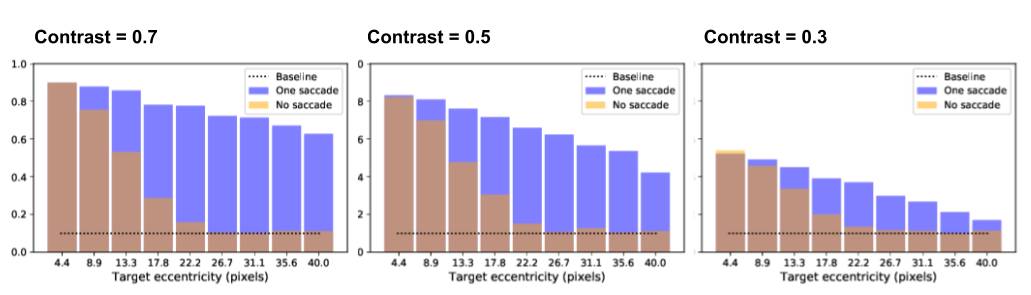
\includegraphics[width=\linewidth]{fig-results-contrast.png}}
	% \includegraphics[]{../../2019-07-15_CNS/figures/CNS-saccade-8.png} % TRUE
	\caption{
		{\bf Effect of contrast and target eccentricity.} %
		The active vision agent is tested for different target eccentricities (in pixels) and different contrasts to estimate a final classification rate. Orange bars: pre-saccadic accuracy from the central classifier ('No saccade') with respect to the target's eccentricity, averaged over $1000$ trials per eccentricity. Blue bars: post-saccadic classification rate. % \if 0\ICANN{\color{blue} TODO: show three levels of noise Low (0.5) median (1.2) high (2). TODO: compare with Accuracy max (knowing the position)}\fi
		\label{fig:results}}%
\end{figure}%


%The result of Figure~\ref{fig:results}-D, correspond to a SNR of $0.7$ and we replicated the result for SNRs of $0.3$ and $0.5$. First, we re-iterated for each SNR the whole process, first by learning the ``what'' pathway, then the accuracy maps and finally the ``where'' pathway.


To test the robustness of our framework, the same experiment was repeated at different signal-to-noise ratios (SNR) of the input images. Both pathways being interdependent, it is crucial to disentangle the relative effect of both sources of errors in the final accuracy. By manipulating the SNR and the target eccentricity, one can precisely monitor the network detection and recognition capabilities, with a detection task ranging from ``easy'' (small shift, strong contrast) to ``highly difficult'' (large shift, low contrast). The digit recognition capability is systematically evaluated in Figure~\ref{fig:results} for different eccentricities and different SNRs.
%in simulation as the average accuracy obtained at the landing of the predicted saccade (see). For each different visual display (a different digit at a different position with a different noise clutter), a retinocentric visual input is processed (figure~\ref{fig:results}-A), providing a predicted accuracy map (figure~\ref{fig:results}-B) that can be compared to the actual future accuracy. Then, a saccade is carried out based on the most probable position as computed from the predicted accuracy map (figure~\ref{fig:results}-C), and the final accuracy is computed from the ``what'' pathway using LeNet model.
For 3 target contrasts conditions ranging from 30\% to 70\% of the maximal contrast, and 10 different eccentricities ranging from 4 to 40 pixels, the final accuracy is tested on $1,000$ trials both on the initial central snippet and the final central snippet (that is, at the landing of the saccade).
The orange bars provide the initial classification rate (without saccade) and the blue bars provide the final classification rate (after saccade) -- see figure~\ref{fig:results}. As expected, the accuracy decreases in both cases with the eccentricity, for the targets become less and less visible in the periphery. The decrease is rapid in the pre-saccadic case: the accuracy drops to the baseline level for a target distance of approximately $20$ pixels from the center of gaze. The post-saccadic accuracy has a much wider range, with a slow decrease up to the border of the visual display (40 pixels away from the center).
When varying the target contrast, the pre-saccadic accuracy profile is scaled by the reference accuracy (obtained with a central target), whose values are approximately $92\%$, $82\%$ and $53\%$ for contrasts of $70$, $50$ and $30$\%. The post-saccadic accuracy profile undergoes a similar scaling at the different contrast values, indicating the critical dependence of the global setup to the central processing reliability.

%yet with the scaling imposed by the ``What'' pathway. This contrast-dependent scaling shows a global dependence of the full setup on the central the robustness of our framework to the different factors of difficulty.

The high contrast case (see fig.~\ref{fig:results}) provides the greatest difference between the two profiles, with an accuracy approaching $90\%$ at the center and $60\%$ at the periphery. This allows to recognize digits after one saccade in a majority of cases, up to the border of the image, from a very scarce peripheral information. This full covering of the 128$\times$128 image range is done at a much lesser cost than would be done by a systematic image scan, as in classic computer vision\footnote{Consider the processing cost (lower bound) as linear in the size of the visual data processed, as it is established in classic computer vision. Taking $n$ the number of pixels in the original image, our log-Polar encoding provides $O(\log n)$ log-polar visual features by construction. The size of the visual data processed is the addition of the $C$ pixels processed at the fovea and the $O(\log n)$ log-polar visual features processsed at the periphery. The total processing cost is thus $O(C+\log n)$. This cost is to be contrasted with the $O(n)$ processing cost found when processing all the pixels of the original image.
}.
With decreasing target contrast, a general decrease of the accuracy is observed, both at the center and at the periphery, with about 10\% decrease with a contrast of $0.5$, and $40\%$ decrease with a contrast of $0.3$. In addition, the proportion of false detections also increases with contrast decrease. At $40$ pixels away from the center, the false detection rate is approximately $40\%$ for a contrast of $0.7$, $60\%$ for a contrast of $0.5$ and $80\%$ for a contrast of $0.3$ (with a recognition close to the baseline at the periphery in that case). The difference between the initial and the final accuracies is maximal for eccentricities ranging from $15$ to $30$ pixels. This optimal range reflects a proportion of the visual field around the fovea where the target detection is possible, but not its identification. The visual agent knows \emph{where} the target is, without exactly knowing \emph{what} it is.

% energy consumption

%The benefit of active inference can be enhanced by doing several saccades.

%As our saccade selection algorithm may implement the essential operations done in the ``Where'' pathway, the central classifier may also reflect the response of the ``What'' pathway, giving the potential category of the digit.

\subsection{Closed-loop setup}

In our simulation results, the post-saccadic accuracy is found to overtake the pre-saccadic accuracy \emph{except} when the target is initially close to the center of gaze. When closely inspecting the 1-10 pixels eccentricity range in our first experiment (not shown), a decision frontier between a positive and a negative information gain is found at 2-3 pixels away from the center. Inside that range, no additional saccade is expected to be produced, and a categorical response should be given instead. %(see figure~\ref{fig:center}), %between the first and the second spatial scale,
It is crucial here to understand that this empirical accuracy difference can be predicted, by construction, as the difference of the maximal outputs of the Where and the What pathways. This difference-of-accuracies prediction can serve as a decision criterion before actuating the saccade, like a GO/NOGO signal. It is moreover interpretable as an approximation of the information gain provided by the ``Where'' pathway, with the true label log-posterior seen as a sample of the posterior entropy -- see eq.(\ref{eq:IG} in section~\ref{sec:IG}).


After a first saccade, while the decision criterion is not attained, additional saccades may be pursued in order to search for a better centering.
In the false detection case for instance, the central accuracy estimate should be close to the baseline, and may allow to ``explain away'' the current center of gaze and its neighborhood, encouraging to actuate long-range saccades toward less salient peripheral positions, making it possible to escape from initial prediction errors.
This incitement to select a saccade ``away'' from the central position is reminiscent of a well-known phenomenon in vision known as the ``inhibition of return''~\cite{Itti01}.
%As a matter of fact, our dual-pathway network is capable to perform such a sequence without any additional
Combining accuracy predictions from each pathway may thus allow to refine saccades selection in a way that complies with the sequential processing observed in biological vision\footnote{Extended to a multi-target case, the Information Gain maximization principle still holds as a general measure of scene understanding improvement through multiple saccades. It is uncertain however wether biologically realistic implementations would be possible in that case.}.
%Our main argument is that such an accuracy map is trainable in a rather straightforward way,
%More generally, this decision principle relies on an interpretation of the Information Gain metric as a difference between central and peripheral accuracy processing.
%Such heuristic also gives a principled formulation of the inhibition of return mechanism which is an important aspect for modeling saccades~\cite{Itti01}.
In particular, we predict that such a mechanism is dependent on the class of inputs, and would be different for searching for faces as compared to digits

% {\color{red} \textbf{Rev 2} What about inhibition of return? Does your model implement it? What prevents your model to jump to a previously foveated position? }

Some of the most peripheral targets are thus difficult to detect in just one saccade, resulting in degraded performances at the periphery (see Figure~\ref{fig:results}). Even when correctly detected, our log-polar action maps also precludes precise centering. As a consequence, peripheral targets are generally poorly centered after the first saccade, as shown for instance in figure~\ref{fig:saccades}-D, resulting in classification errors. The possibility to perform a sequential search using more saccades is thus crucial to allow for a better recognition.
Results on multi-saccades visual search results are presented in figure~\ref{fig:results-saccades}.


%: see Figure~\ref{fig:results}
\begin{figure}[t!]%%[p!]
	%\flushleft{\bf (A) \hspace{4.2cm} (B) \hspace{2cm} (C) \hspace{4cm} (D)\hspace{6cm}}
	\centering{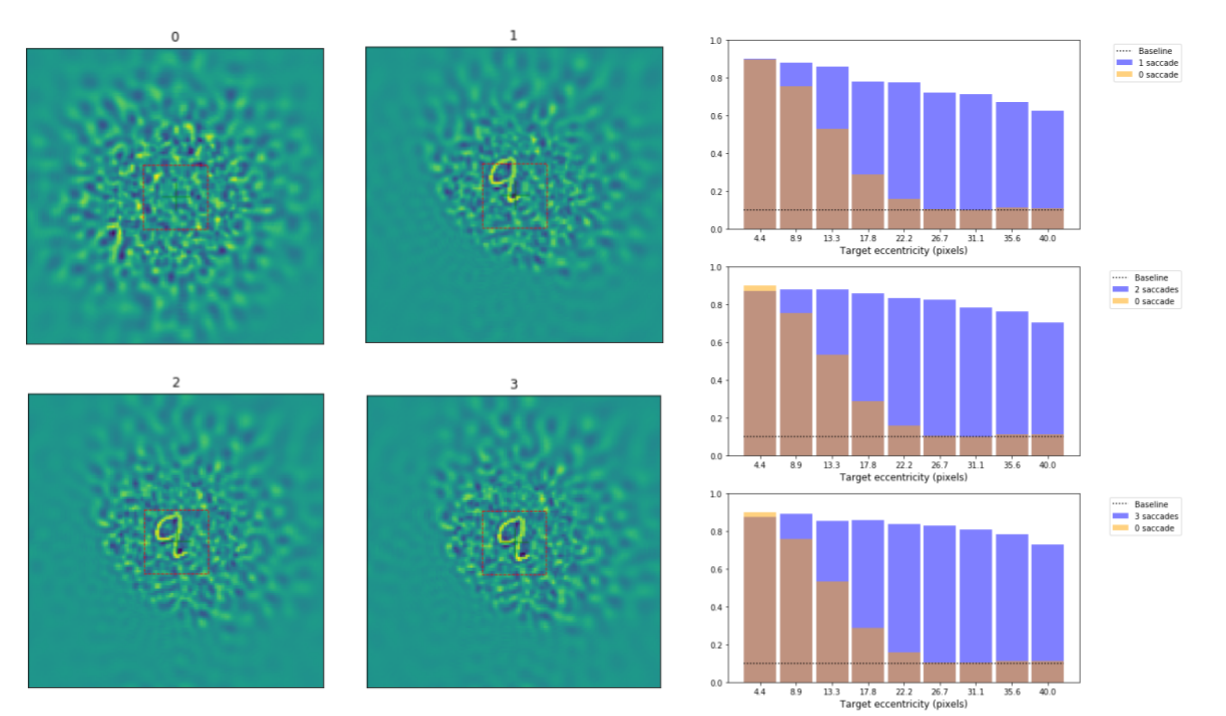
\includegraphics[width=\linewidth]{fig-results-saccades.png}}
	% \includegraphics[]{../../2019-07-15_CNS/figures/CNS-saccade-8.png} % TRUE
	\caption{
		{\bf Closed-loop setup.} %
		\A Example of a trial with a sequence of 3 saccades. The subjective visual field is reconstructed from the log-polar visual features, with red square delineating the $28\times28$ foveal snippet, after 0, 1, 2 and 3 saccades (from left to right). After the first saccade, the accuracy predicted by the ``Where'' network is higher than that predicted by the ``What'' network and a corrective saccade is realized to center the target. After this saccade, the foveal accuracy is higher than that predicted in the periphery and the answer \ANS\ is given. % TODO : on pourrait mettre le carré central d'une autre couleur pour dire que What ``gagne''
		\B Average classification accuracies measured for different target eccentricities (in pixels) and a different number of saccades. Target contrast set to $70\%$. Orange bars: pre-saccadic central accuracy (``0 saccade'') with respect to eccentricity, averaged over $1000$ trials per eccentricity. Blue bars: Final classification rate after one, two and three saccades (from left to right, respectively).
		\label{fig:results-saccades}}%
\end{figure}%

An example of a trial with a sequence of 3 saccades is shown on figure~\ref{fig:results-saccades}-A. A hardly visible peripheral digit target is first approximately shifted to the foveal zone thanks to the first saccade. Then, a new retinal input centered at the new point of fixation is computed, such that it generates a novel predicted accuracy map. The second saccade allows to improve the target centering. As the predicted foveal accuracy given by the ``What'' network is higher than the peripheral one given by the ``Where'' network, a third saccade would not improve the centering: The stopping criteria is met.
%Interestingly, this shows that the competition between both networks (see section~\ref{sec:IG}) is suffficient to implement a closed loop sequence, without needing to include an inhibition of return heuristic.
In practice, 1 or 2 saccades were sufficient in most trials to reach the actual target.
%, and then that the accuracy of the answer was only dependent to that of the ``What'' classifier.
Another behavior was also observed for some ``bad start'' false detection cases (as in figure~\ref{fig:saccades}-C for instance), when the target is shifted away in the opposite direction and the agent can not recover from its initial error. From figure~\ref{fig:results-saccades}-B, this case can be estimated at about $15\%$ of the cases for the most peripheral targets.

% TODO : à la place, je mettrais soit une stratégie open-loop=1 sacade, soit une stratégie closed-loop qui continue tant que la condition d'arrêt n'est pas remplie. on donne alors les pourcentage du nombre de saccades nécessaires pour atteindre le stopping criterium (ma prédiction= 1:85% 2:10% 3et+:5%)
Overall, as shown in figure ~\ref{fig:results-saccades}-B, the corrective saccades implemented in this closed-loop setup provide a significant improvement in the classification accuracy. Except at the center, the accuracy increases by about $10\%$ both for the mid-range and the most peripheral eccentricities. Most of the improvement however is provided by the first corrective saccade. The second corrective saccade only shows a barely significant improvement of about $2\%$ which is only visible at the periphery. The following saccades would mostly implement target tracking, without providing additional accuracy gain. A 3-saccades setup finally allows a wide covering of the visual field, providing a close to central recognition rate at all eccentricities, with the residual peripheral error putatively corresponding to the ``bad start'' target misses cases.
